\section{Entorno de Desarrollo Local}

Para garantizar la reproducibilidad del proyecto, en esta sección se descibirá el entrono de desarrollo en el que se ha realizado y el acceso al repositorio con el código fuente.

\subsection{Tecnologías y Versiones}

El proyecto se ha desarrollado en un entorno \textbf{Windows 10}, aunque esto no influye en la compatibilidad, ya que todas las tecnologías utilizadas son multiplataforma, lo cual permite realizar el desarrollo en cualquier sistema operativo sin restricciones. En la tabla \ref{tab:dependencias_versiones} se presentan las tecnologías principales empleadas en el proyecto junto con sus versiones correspondientes.

\begin{table}[htbp]
    \centering
    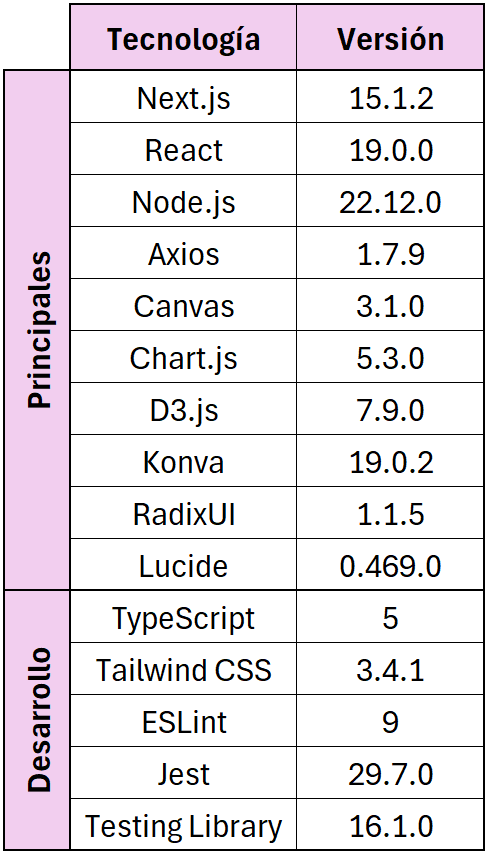
\includegraphics[width=0.37\textwidth]{figures/dependencias_versiones.png}
    \captionsetup{skip=5pt}
    \caption{Dependencias usadas en el desarrollo, junto con sus versiones.}
    \label{tab:dependencias_versiones}
\end{table}

Cabe destacar que el gestor de paquetes utilizado en el proyecto ha sido \textbf{\texttt{pnpm} (\textit{Performant Node Package Manager})}, en lugar de \texttt{npm} (\textit{Node Package Manager}) o \texttt{yarn} (\textit{Yet Another Resource Negotiator}). La elección de \texttt{pnpm} se debe a sus mejoras en la gestión de dependencias y optimización del uso del espacio de almacenamiento. A diferencia de \texttt{npm}, \texttt{pnpm} utiliza un sistema de enlaces en lugar de duplicar archivos en cada proyecto, lo que reduce significativamente el consumo de espacio. Además, \texttt{pnpm} es completamente compatible con los paquetes del registro de \texttt{npm}, lo que garantiza su interoperabilidad con la mayoría de los ecosistemas de desarrollo basados en \textit{Node.js}.

\subsection{Instalación y Configuración del Proyecto}

El proyecto se encuentra alojado en un repositorio de \textit{GitHub}\footnote{Repositorio del proyecto: \href{https://github.com/jonortega/tfg-app-spotify}{https://github.com/jonortega/tfg-app-spotify}} para evitar pérdidas y tener disponibilidad completa al código. Para ejecutarlo localmente, además de haber instalado \textit{Node.js}, hay que clonar el respositorio, acceder a la carpeta y ejecutar los comandos de instalación y ejecución. A continuación, se muestran los comandos necesarios para realizar estos pasos:

\begin{ifalgorithm}[H]
    \begin{lstlisting}[language=bash]
    # Clonar el repositorio
    git clone https://github.com/jonortega/tfg-app-spotify.git
    
    # Acceder al directorio del proyecto
    cd tfg-app-spotify
    
    # Instalar dependencias
    pnpm install
    
    # Ejecutar el servidor de desarrollo
    pnpm run dev
    \end{lstlisting}
    \caption{Comandos de instalación y ejecución inicial del proyecto.}
    \label{alg:instalacion_proyecto}
\end{ifalgorithm}

Tras estos pasos, la página web estará accesible en \texttt{localhost:3000}. Es encesario agregar un fichero de variables de entorno \texttt{.env.local}, ya que, por seguridad, no se registra en el sistema de control de versiones. El contenido de dicho fichero se muestra en el \hyperref[alg:variables_entorno]{Anexo C}.

Dos de las variables de entorno necesarias para poder tratar con la API de \textit{Spotify}, son el \textbf{Client ID} y el \textbf{Client Secret}. Estos dos valores se obtienen al realizar el registro de la aplicación en la plataforma de desarrollo de \textit{Spotify}. En la siguiente sección, se explicará cómo realizar este registro y dónde obtener dichas variables.

\section{Registro de la Aplicación en Spotify}

\section{Ciclo de Vida del Desarrollo}

\subsection{Incremento I: Prototipado Rápido}

\subsection{Incremento II: Producto Mínimo Viable (PMV)}

\subsection{Incremento III: Producto Final}

\section{Implementación del Fronted}

\subsection{Lógica de las Estadísticas}

\subsection{React Hooks}

\section{Implementación del Backend}

\subsection{Lógica y Tratamiento de Datos en el Servidor}

\subsection{Estructuras de Datos}

\section{Optimizaciones}